%to build: "pdflatex report.tex"

%\documentclass[journal]{IEEEtran}
\documentclass{article}
\usepackage{amsmath}
\usepackage{listings}
\usepackage{graphicx}
\usepackage{multicol}
\usepackage{wrapfig}
\graphicspath{./imgs/}
\DeclareGraphicsExtensions{.pdf, .jpeg, .png}
\usepackage{geometry}
\geometry{a4paper, portrait, margin=1in}

\newcommand{\includecode}[2][c]{\lstinputlisting[caption=#2, escapechar=, language=#1]{#2}}
 
\hyphenation{op-tical net-works semi-conduc-tor}
\begin{document}

\title{Computational Physics Midterm Project}
\author{
Austin~F.~Oltmanns
\and
Noah~Seekins
}

\maketitle

% As a general rule, do not put math, special symbols or citations
% in the abstract or keywords.
\begin{abstract}
Ray-tracing techniques are explored for the purpose of rendering 3d scenes which contain meshes made of
triangular sections of planer surfaces. Linear algebra techniques are used to obtain computationally 
efficient methods. It is shown that shadows are simulated using this method, which is an improvement 
from rendering techniques previously explored in the class.
\end{abstract} 

\section{Introduction}
%\IEEEPARstart{T}{his}
This midterm assignement required students to design and develop a simulation of a physical phenomenon 
of their choosing. Our group chose to explore ray-tracing because we felt it aligned closely with the 
material presented in class thus far and also presented a complex enough subject to warrent exploration.
The system implemented shows a triangular section casting a shadow onto a ground plane from light sources
present above the triangular surface (above meaning in the +Z direction of the world's coordinates).

To perform this experiment, light rays are traced starting from their end point inside the camera, out through
a pinhole, reflected a number of times off of the world, and back to either a light source or found to not 
reach a light source.

For simplicity, real world units have been disregarded in an effort to keep the numbers used in the simulation from 
becoming very large or small (which can affect the stability of the simulation).
Each aspect of the simulation will be described in detail below and the code is attached as an appendix to this report.

\section{Ray Generation}
\subsection{Description}
%ORDER
The first step is to determine the end point of each ray inside the camera. These end points correspond to 
pixels displayed on the screen and the color of each pixel is an average of the color of each ray which ends
at that point. This implies that for each pixel, there must be a sufficient number of rays which terminate
at that point. To determine each of these rays' origin points and directions in the world coordinate system,
a transform from the imaging plane of the camera (the "film") to the world is created based on parameters from the camera.

%%%
%Figure of plane with vectors pointing to the pinhole
%%%
\begin{figure}[!t]
\centering
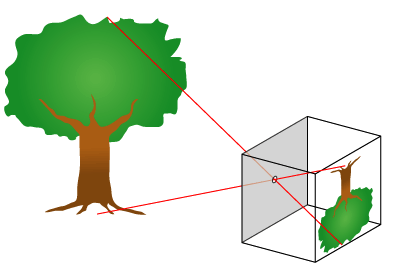
\includegraphics[width=3.5in]{./imgs/Pinhole-camera}
\caption{The rays are shown in this figure as the red lines. Note how each ray passes through the pinhole
of the camera from the imaging plane and into the world. (Public Domain)}
\label{fig:pinhole}
\end{figure}

Fig.~\ref{fig:pinhole} shows two rays begining (ending) at the imaging plane and passing through the pinhole
of the virtual camera. What is not shown is how the rays reflect off of objects in the world to arrive
 (or not arrive) at light sources.

\subsection{Implementation}
If the axes which define the coordinates system with its origin at the pinhole of the camera and 

\subsection{Coordinate Transform}
\begin{figure}[!t]
\centering
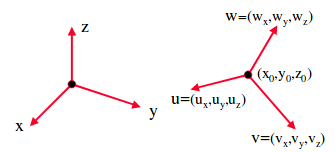
\includegraphics[width=3.5in]{./imgs/axes}
\caption{World and camera axes together. Camera axes have been defined with reference to the world axes.}
\label{fig:axes}
\end{figure}


lots of coordinates and stuff
%describe the camera coordinate systema and the transform between it and the world coordinate system. 
%describe that the rays origin points are just the center of each pixel on the imageing plane
%so the rays are just the rays which start at that point and point towards the pinhole

\section{Ray interaction with World}
\subsection{Description}
making sure the rays bounce off of stuff

\subsection{Implementation}

description of math

\section{Conclusion}
Obviously there are approximations which take place in a simulation. The question a simulator must ask is how
much approximation is acceptable and how much error can be allowed. The data from these experiments show that this
module should most likely not be used for low temperature collisions of groups of gas particles. However, at higher
temperatures the resuslts could be acceptable depending on application.

Additionally, the 3D rendering system outlined in this report is very modular and could be extended easily to 
do things like having the camera follow a path or track certain elements throughout the simulation.

The code used to complete this assignment is attached as an appendix to this document.

\section{References}
links to ray tracing guide

%https://en.wikipedia.org/wiki/Pinhole_camera_model

\newpage
\onecolumn
\section{Appendix}
\lstinputlisting[language=c]{../src/main.c}
\lstinputlisting[language=c]{../src/renderer.c}
\lstinputlisting[language=c]{../src/triangleSurface.c}
\end{document}